\chapter{Analisi Statica}

L'obiettivo generale della sicurezza del software è prevenire, rilevare e mitigare le 
vulnerabilità. L'analisi del codice (sia sorgente che eseguibile) è fondamentale per 
questo scopo:

\begin{itemize}
    \item \textbf{Analisi Dinamica}: Verifica il software eseguendolo con specifici input.
    Esempi di analisi dinamica sono il Testing Funzionale, i Web Application scanner, il
    Fuzzing e il DAST. Il limite intrinseco è che può certificare la sicurezza solo 
    dei percorsi di esecuzione (path) che vengono effettivamente esplorati durante i 
    test.
    \item \textbf{Analisi Statica}: Verifica il software senza eseguirlo, "leggendo" 
    il codice sorgente o binario. Esempi di analisi statica sono: le Code Reviews, le 
    Code Inspection e il SAST. Ha il vantaggio di poter coprire teoricamente tutti i 
    percorsi di esecuzione, inclusi i casi limite o il codice "morto", ma può 
    essere soggetta a imprecisioni generando dei falsi positivi o falsi negativi.
\end{itemize}

\begin{figure}[H]
    \centering
    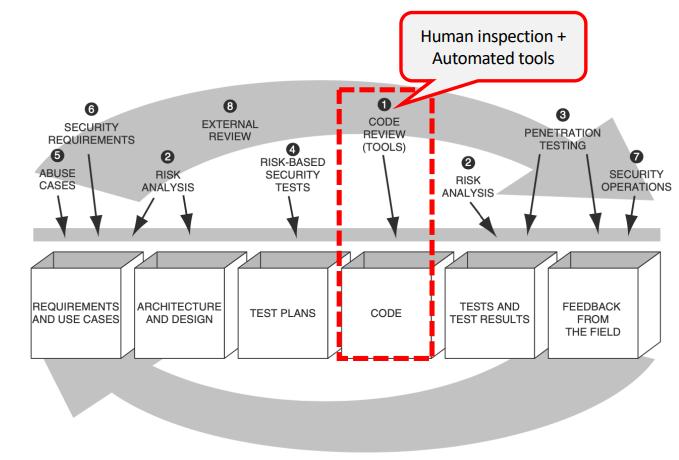
\includegraphics[width=0.9\linewidth]{img/capitolo7/lifecycle.png}
    \label{fig:lifecycle}
\end{figure}

Dalla figura soprastante vediamo che l'analisi statica si posiziona all'interno del 
ciclo di vita della sviluppo del software sicuro fin dalle prime fasi: iniziata la 
stesura del codice del software si combina l'ispezione umana con strumenti automatizzati 
al fine di condurre un'analisi statica di qualità. Questo dimostra che l'analisi 
statica non è una soluzione isolata, ma un componente integrante (idealmente durante 
la fase di codifica) di un approccio metodico alla sicurezza.

Sebbene l'analisi statica manuale sia potenzialmente efficace, tale analisi risulta 
essere purtroppo anche costosa, difficile e soggetta ad errori, ecco perché è importante 
combinare l'ispezione umana con strumenti automatizzati. I tool di analisi statica 
servono a rendere la revisione del codice più veloce e fruttuosa; essi identificano 
potenziali problemi che devono poi essere ulteriormente revisionati dagli sviluppatori.

\section{Tecniche di Base}

\textbf{Type Checking}

Il primo analizzatore statico che un programmatore incontra è il compilatore. 
Linguaggi fortemente tipizzati (Java, C\#) prevengono intere classi di vulnerabilità 
a compile-time, mentre C/C++ sono molto più permissivi. In C infatti è possibile 
ad esempio assegnare una variabile di tipo \textit{int} a una di tipo \textit{short}:

\begin{lstlisting}
int i = ...;
short s = i;
\end{lstlisting}

In C questo è possibile poiché esso lo permette tramite una \textbf{conversione implicita}, mentre 
in Java questo genera un errore di tipi incompatibili.

\textbf{Compiler Warnings}

L'attivazione di avvisi estesi nel compilatore o interprete fin dalle prime fasi di 
sviluppo può prevenire difetti di sicurezza. L'aggiunta dell'opzione \textit{-Wconversion}
nel compilatore gcc ci avrebbe avvisati della conversione implicita vista prima:
\begin{gather*}
    \text{\$ gcc -Wconversion test.c}
\end{gather*}

Esempio del "\textbf{goto fail}" di Apple iOS: questo bug nel codice dell'OS Apple 
riguardava l'implementazione del protocollo TLS/SSL.

\begin{lstlisting}
if ((err = SSLHashSHA1.update(&hashCtx, &signedParams)) != 0)
    goto fail;
    goto fail;  //Eseguito incondizionatamente!
err = sslRawVerify(...) //DEAD CODE
\end{lstlisting}

In C, l'assenza di parentesi graffe nell'istruzione if fa sì che solo la prima 
istruzione \textit{goto fail;} sia condizionata, la seconda istruzione \textit{goto fail;} 
viene sempre eseguita. A livello di sistema, questo fa saltare del tutto il controllo 
crittografico critico \textit{sslRawVerify}; se un attaccante esegue un attacco 
\textit{Man-In-The-Middle} e invia una firma non valida, i controlli precedenti non falliscono 
(err == 0), il codice salta all'etichetta \textit{fail}, e la funzione restituisce 
err (che è 0, ovvero "Successo"). L'attaccante ha così bypassato l'autenticazione.
Un semplice warning del compilatore come \textit{-Wunreachable-code} o \textit{-Wimplicit-fallthrough} 
avrebbe rilevato il codice morto successivo al goto.

\textbf{Style Checkers, Defect Finders e Quality Scanners}

Strumenti come \textbf{PMD} (per il codice sorgente Java) o \textbf{FindBugs} (per il 
bytecode) confrontano il codice con regole predefinite per identificare difetti di 
stile o di qualità strutturale. Ad esempio l'uso dell'operatore "\textit{==}" per 
confrontare due stringhe in Java invece del metodo corretto \textit{x.equals(y)} è un 
errore classico rilevato da questi strumenti. Anche se si concentrano sulla qualità 
generale piuttosto che sulla sicurezza, risolvere questi difetti facilita il lavoro 
degli scanner di sicurezza.

\textbf{Security Defect Text Scanners}

Sono strumenti che funzionano in modo simile al comando \textit{grep}, analizzando 
il testo del codice tramite un lexer molto semplice. Cercano chiamate a funzioni note 
per essere insicure, come copie di stringhe non sicure, generatori di numeri casuali 
deboli o API crittografiche deprecate. Ad esempio l'uso del tool \textit{Flawfinder}
permette di individuare chiamate alla funzione \textit{strncat}, la quale, pur essendo
spesso considerata sicura, viene facilmente usata in modo scorretto portando a 
vulnerabilità.

\section{Tecniche Avanzate e Modellazione}

La pulizia del codice attraverso strumenti di base visti prima è una fase propedeutica 
cruciale. Rimuovere difetti generici e di stile semplifica l'analisi per gli 
strumenti orientati prettamente alla sicurezza, riducendo l'incidenza di falsi 
risultati. I \textit{text scanner}, sebbene siano molto veloci e possano processare 
anche codice parziale o non compilabile, mancano di comprensione del contesto e 
generano molti falsi allarmi, evidenziando il limite delle tecniche di base e 
aprendo la strada a strumenti di analisi più sofisticati.

Gli analizzatori statici avanzati (noti come \textit{Security Defect Finders}) non si 
limitano a cercare parole chiave nel testo come un semplice grep. Essi creano un 
modello interno del programma e analizzano le proprietà di sicurezza su di esso. 
Sebbene richiedano tempi di compilazione più lunghi, offrono un'analisi molto più 
potente e accurata.

\subsection{Modellazione}

Per analizzare il codice profondamente, gli strumenti lo trasformano in strutture 
dati complesse (rappresentazioni intermedie). Le principali sono:

\textbf{Abstract Syntax Tree (AST)}

È la struttura dati fondamentale usata dai compilatori e dagli analizzatori. 
Rappresenta la struttura sintattica del programma ad albero:

\begin{itemize}
    \item \textit{Nodi}: Rappresentano gli elementi del programma (es. dichiarazioni, assegnazioni, espressioni matematiche).
    \item \textit{Archi}: Collegano gli elementi ai loro sotto-elementi (es. un nodo di assegnazione avrà due figli: il valore a destra e la variabile a sinistra).
\end{itemize}

\begin{lstlisting}
int homer(int x){
    int y, a, b;
    if(x>0){
        y = 0;
    } else{
        a = bart(1);
        b = lisa(2);
        y = a + b;
    }
    return y;
}
\end{lstlisting}

Nell'esempio riportato l'AST del metodo \textbf{homer} sarà così composto:

\begin{itemize}
    \item 1 nodo radice per la dichiarazione del metodo \textbf{homer}.
    \item 4 nodi figli per il \textit{return type (int)}, \textit{method name (homer)},
    dichiarazione delle variabili in input \textit{(int x)} e il corpo del metodo.
    \item 3 nodi figli aventi come genitore il nodo che rappresenta il corpo del metodo;
    i nodi figli in particolare denotano la dichiarazione di variabili \textit{(int y, a, b)},
    una condizione if \textit{(if(x>0) then ... else ...)} e un \textit{return (return y)}.
    \item La costruzione dell'albero continua ricorsivamente...
\end{itemize}

\begin{figure}[H]
    \centering
    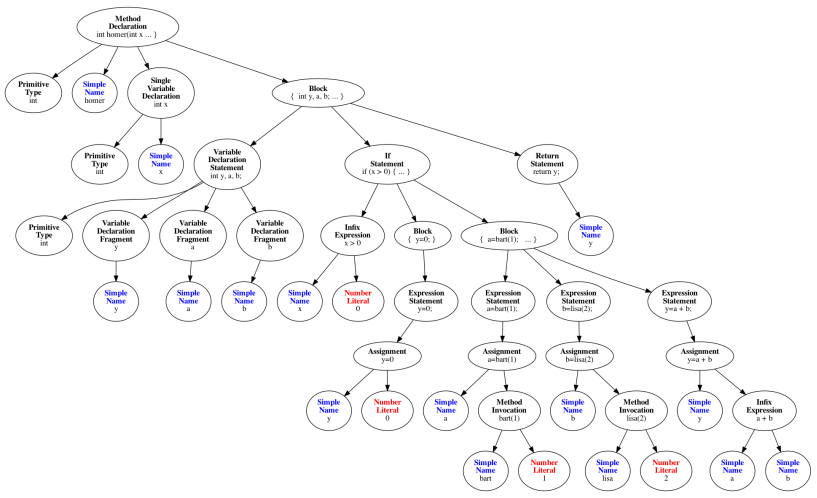
\includegraphics[width=1\linewidth]{img/capitolo7/ast.png}
    \label{fig:ast}
\end{figure}

\textbf{Grafi Avanzati}

Partendo dall'AST, vengono generati grafi più sofisticati per capire come i dati e le 
istruzioni si muovono:

\begin{itemize}
    \item \textbf{Control Flow Graph (CFG)}: Rappresenta i percorsi di esecuzione del 
    programma (i blocchi di codice e i rami come if/else).
    \item \textbf{Call Graph}: Mostra quali funzioni chiamano quali altre funzioni 
    (es. \textit{main} chiama \textit{homer}, che a sua volta chiama \textit{bart} e \textit{lisa}).
    \item \textbf{Program Dependency Graph (PDG)}: Mappa le dipendenze dei dati (es. 
    dove una variabile viene scritta e dove viene letta) e del controllo.
\end{itemize}

\begin{figure}[H]

\begin{subfigure}{0.5\textwidth}
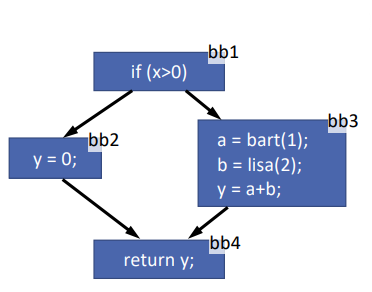
\includegraphics[width=0.9\linewidth]{img/capitolo7/cfg.png} 
\caption{CFG}
\label{fig:CFG}
\end{subfigure}
\begin{subfigure}{0.5\textwidth}
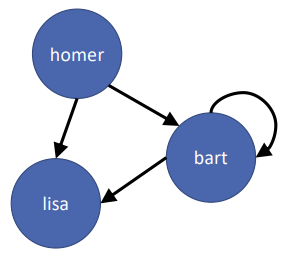
\includegraphics[width=0.9\linewidth]{img/capitolo7/call.png}
\caption{Call Graph}
\label{fig:CallGraph}
\end{subfigure}
\begin{subfigure}{0.5\textwidth}
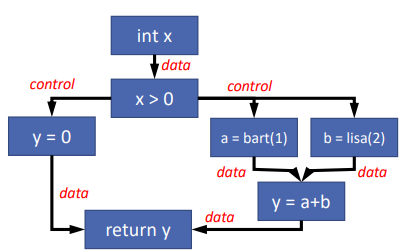
\includegraphics[width=0.9\linewidth]{img/capitolo7/pdg.png}
\caption{PDG}
\label{fig:PDG}
\end{subfigure}
\label{fig:grafi}
\end{figure}

\subsection{Tipologie di Analisi di Sicurezza Avanzata}

Basandosi su questi modelli, gli analizzatori possono eseguire controlli sofisticati:

\textbf{Taint Propagation Analysis}

È una forma di analisi del flusso di dati che traccia il percorso delle informazioni 
da fonti non attendibili ("\textit{Sources}") fino a funzioni critiche per la sicurezza 
("\textit{Sinks}").

\begin{lstlisting}
                               (*@$\downarrow$@*)//Source                     
if( fgets(buf, sizeof(buf), stdin) == buf ) {
    strcpy( other, buf );
    system( other );
}             (*@$\uparrow$@*)//Sink
\end{lstlisting}

Nell'esempio riportato sopra, un input utente viene letto tramite \textit{fgets} e 
inserito nella variabile \textit{buf} (\textbf{Source}, il dato diventa "tainted", 
ovvero "sporco/infetto"). Il dato poi viene passato ad un'altra variabile \textit{other}
tramite la funzione \textit{strcpy}. Infine, la variabile \textit{other} viene passata
alla funzione \textit{system()} (\textbf{Sink}); l'analizzatore collega questi punti 
e segnala una vulnerabilità di "\textit{OS command injection}".

\textbf{Range Analysis}

Verifica l'intervallo di valori potenziali che una variabile può assumere. È 
fondamentale per prevenire i Buffer Overflow.

\begin{lstlisting}
char buf[10];
strcpy(buf, "hello");
strcat(buf, "world!");
\end{lstlisting}

Compilando il codice soprastante con l'opzione \textit{-fanalyze} otteniamo un warning
di \textit{stack-based buffer overflow}, questo perché il compilatore sa che \textit{buf} ha 
una capacità di 10 byte sullo stack. La funzione \textit{strcpy} scrive 6 byte (hello$\backslash$0),
successivamente la funzione \textit{strcat} concatena 7 byte (world!$\backslash$0)
sovrascrivendo a partire dal terminatore. Il totale è quindi 12 caratteri + 1 terminatore 
= 13 byte, l'analizzatore statico calcola queste dimensioni a compile-time e segnala 
il CWE-121 (Buffer Overflow).

\textbf{Type State Analysis}

Verifica che le operazioni eseguite su un oggetto rispettino un "protocollo" o una 
specifica macchina a stati (es. inizializzato $\rightarrow$ usato $\rightarrow$ liberato).

\begin{lstlisting}
while ((node = *ref) != NULL) {
    *ref = node->next;
    free(node); //L'oggetto passa allo stato "freed"
    // ERRORE: Manca "node = NULL;"
    if (!unchain(ref)) {
        goto ERROR;
    }
}
ERROR:
if (node != NULL) {
    free(node); // Vulnerabilita: Double free!
    return UNCHAIN_FAIL;
}
\end{lstlisting}

Nell'esempio riportato il puntatore \textit{node} viene passato a \textit{free()}, lo 
stato dell'oggetto diventa "\textbf{freed}". Tuttavia, il puntatore \textit{node} non 
viene impostato a \textit{NULL}. Se la funzione \textit{unchain} fallisce, il codice 
salta all'etichetta \textit{ERROR}. Qui, il controllo \textit{node != NULL} risulta 
ancora vero e viene invocata nuovamente \textit{free(node)}. L'analizzatore, seguendo 
la macchina a stati, capisce che il nodo era già nello stato "\textbf{freed}" e segnala una 
vulnerabilità di "\textit{Double Free}".

\section{Astrazione e Zero Analysis}

Per analizzare in modo esaustivo un programma, un analizzatore statico non può 
semplicemente simulare l'esecuzione tenendo traccia di ogni singolo valore esatto 
che una variabile può assumere. Le combinazioni possibili (lo spazio degli stati) 
sarebbero pressoché infinite, e l'analisi richiederebbe secoli. La soluzione a questo 
problema è l'\textbf{Astrazione}.

L'astrazione è il processo attraverso il quale l'analizzatore statico "semplifica" 
la realtà del programma. Invece di tracciare i valori esatti (\textit{concrete domain}), 
l'analizzatore mappa i dati su un dominio semplificato (\textit{abstract domain}), 
concentrandosi solo sulle proprietà che gli interessano per trovare specifici bug.
Se ad esempio abbiamo una variabile intera $n$, invece di chiederci il valore esatto di
$n$, l'analizzatore si chiede il segno di $n$. Il dominio astratto diventa quindi semplicemente:
\{Positivo, Negativo, Zero, Sconosciuto\}. Questo espediente riduce drasticamente i 
calcoli necessari, permettendo allo strumento di analizzare milioni di righe di 
codice in tempi ragionevoli.

La \textbf{Zero Analysis} è l'esempio per eccellenza dell'uso dell'astrazione. Il 
suo obiettivo è prevenire una vulnerabilità classica che causa il crash del programma: 
la \textbf{divisione per zero}. Nell'astrazione della Zero Analysis, ogni variabile 
numerica viene etichettata con uno di questi stati astratti:

\begin{itemize}
    \item \textbf{Z (Zero)}: Il valore è sicuramente nullo.
    \item \textbf{NZ (Non-Zero)}: Il valore è sicuramente diverso da zero.
    \item \textbf{T (Sconosciuto)}: Il tool non sa se il valore sia zero o meno.
\end{itemize}

\begin{lstlisting}
int y = getUserInput();    // L'analizzatore etichetta 'y' come 'T' 
int x = 10;                // L'analizzatore etichetta 'x' come 'NZ' 
if (y != 0) {
    // In questo blocco, l'analizzatore AGGIORNA lo stato di 'y' a 'NZ'
    int result = x / y;    // Operazione: NZ / NZ. Risultato: SICURO 
} else {
    // In questo blocco, l'analizzatore AGGIORNA lo stato di 'y' a 'Z'
    int result = x / y;    // Operazione: NZ / Z. Risultato: VULNERABILITA RILEVATA!
}
int z = x / y;            // Fuori dall'if, 'y' torna a essere 'T'. 
                          // Operazione: NZ / T. Risultato: WARNING (Possibile divisione per zero)
\end{lstlisting}

L'astrazione ha un prezzo: semplificando i dati, l'analizzatore perde informazioni. 
Quando l'analizzatore perde troppe informazioni, le variabili finiscono nello stato 
\textbf{T} (Sconosciuto). Quando un analizzatore vede un'operazione critica (come una 
divisione) con una variabile in stato \textbf{T}, per motivi di sicurezza genererà un 
avviso (\textit{Warning}). Se nella realtà dell'esecuzione quel valore non sarebbe 
mai stato zero, l'analizzatore ha appena generato un \textbf{Falso Positivo}.
Più il dominio astratto è semplice, più l'analisi è veloce, ma genererà moltissimi 
falsi positivi. Più il dominio astratto è complesso (tracciando relazioni matematiche 
precise), più l'analisi sarà accurata, ma rischierà di esaurire la memoria o il 
tempo a disposizione.

Vulnerabilità come le divisioni per zero o la dereferenziazione di puntatori nulli, 
che usa la stessa esatta logica della Zero Analysis: puntatore \textbf{Null}, 
\textbf{Non-Null} o \textbf{T}, possono essere sfruttate dagli attaccanti per 
causare attacchi di tipo \textit{Denial of Service} (DoS), facendo crashare 
deliberatamente le applicazioni.

\section{Limiti Teorici e Pratici}

L'analisi statica è sempre soggetta a imperfezioni, essa produce \textbf{falsi allarmi} 
e, soprattutto, genera \textbf{errori mancati} (vulnerabilità reali che lo strumento 
non "vede"). Una regola d'oro della sicurezza è che l'assenza di errori riportati non 
significa che il codice sia privo di errori. Queste imperfezioni sono causate da due 
grandi categorie di problemi:

\textbf{1. Limiti Pratici (Scalabilità e Complessità)}

Analizzare a fondo un software reale richiede una quantità enorme di memoria e 
potenza di calcolo; l'analisi \textit{Intra-procedurale}, che valuta una singola 
funzione isolata, è veloce ma cieca rispetto a ciò che accade fuori da essa. L'analisi 
\textit{Inter-procedurale}, che traccia il flusso di dati tra funzioni diverse, è 
estremamente difficile da scalare su milioni di righe di codice. 

Per far sì che un'analisi termini in tempi ragionevoli, gli analizzatori devono usare 
delle approssimazioni, ignorando in parte il contesto di esecuzione o l'ordine delle 
istruzioni, tramite approcci \textit{Context-insensitive} o \textit{Flow-insensitive}.
Precisione, profondità e scalabilità non possono essere massimizzate contemporaneamente:

\begin{figure}[H]
    \centering
    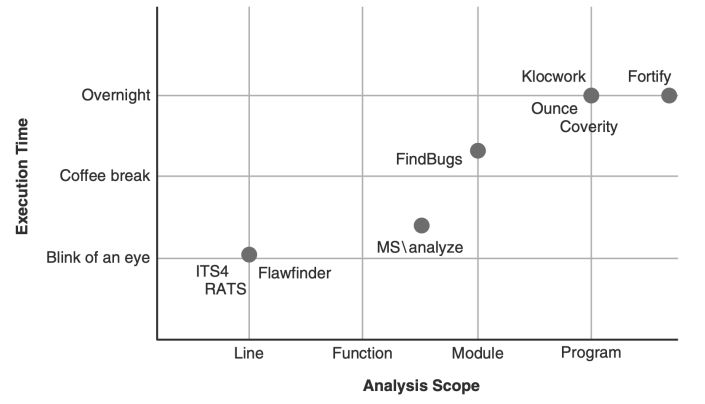
\includegraphics[width=1\linewidth]{img/capitolo7/limiti.png}
    \label{fig:limiti}
\end{figure}

\textbf{2. Limiti Teorici}

L'analisi statica è \textbf{matematicamente indecidibile}: non esiste e non può 
esistere un algoritmo capace di analizzare \textit{tutti} i possibili programmi, con 
\textit{tutti} i possibili input, prevedendone il comportamento in un tempo finito.
Questo limite deriva direttamente dal teorema di Turing; risolvere perfettamente 
l'analisi statica equivarrebbe a risolvere il \textbf{Problema della Fermata} 
(\textit{Halting Problem}), cosa matematicamente impossibile.

Visto che l'analisi statica perfetta non esiste, per renderla utile dobbiamo 
accettare dei compromessi: rilassiamo gli obiettivi accettando che gli strumenti 
approssimino la realtà. Comprendiamo dunque che un tool di SAST non garantisce la sicurezza
assoluta; è necessario allora abbracciare l'approccio di \textbf{Defense in Depth} 
affiancando all'analisi statica i test dinamici (DAST), revisioni manuali (Code Review)
e test di penetrazione.

\section{Analisi statica e gli LLM}

Gli analizzatori statici tradizionali sono ottimi per tracciare flussi di dati e 
trovare vulnerabilità note, ma sono ciechi rispetto al contesto; non sanno a cosa 
serve il programma, chi dovrebbe usarlo e quali sono le regole di business.

Gli LLM sono in grado di incorporare e comprendere un contesto molto più ampio. 
Possono analizzare:

\begin{itemize}
    \item \textbf{L'uso previsto}: Capire \textit{cosa} dovrebbe fare un componente.
    \item \textbf{Modello di controllo degli accessi}: Capire \textit{chi} ha i permessi per fare cosa.
    \item \textbf{Threat Modeling}: Capire da \textit{dove} provengono gli input non attendibili
    e quali sono i reali confini di sicurezza dell'applicazione.
\end{itemize}

Questo rende gli LLM eccezionali per trovare vulnerabilità nella \textbf{Business Logic}, 
ovvero difetti che non derivano da un errore di sintassi o da una funzione non sicura, 
ma da un errore concettuale nella progettazione del software.

Gli analizzatori statici generano moltissimi Falsi Positivi, spesso questo accade 
perché l'analizzatore non riconosce una funzione di sanitizzazione personalizzata 
o perché un percorso di codice è teoricamente vulnerabile ma praticamente 
irraggiungibile da un attaccante. In questo scenario gli LLM vengono allora usati per 
fare il \textbf{Triage} degli avvisi: ad esempio un LLM può analizzare un alert per 
una vulnerabilità XSS; leggendo il codice, l'LLM capisce che la variabile \textit{redirectUrl}
viene accuratamente validata prima dell'uso tramite una funzione che controlla 
\textit{hostname}, \textit{protocol} e \textit{pathname}. L'LLM chiude l'alert classificandolo 
correttamente come \textbf{False Positive}.

Gli LLM sono in grado di condurre un'analisi statica autonoma divisa in fasi:

\begin{enumerate}
    \item \textbf{Context Gathering}: L'agente mappa l'applicazione identificando 
    componenti, entry point e azioni degli utenti, salvando tutto in un database.
    \item \textbf{Issue Suggestion}: Basandosi sul contesto raccolto e sui file come 
    \textit{README.md}, l'LLM ipotizza quali potrebbero essere i rischi principali 
    per quel tipo specifico di app (es. un pannello di admin è a rischio XSS o CSRF).
    \item \textbf{Issue Audit}: L'LLM controlla effettivamente il codice sorgente 
    per verificare se le vulnerabilità ipotizzate esistono davvero, assicurandosi 
    che lo scenario di attacco sia realistico e non richieda privilegi di 
    amministratore preesistenti.
    \item \textbf{Filtering}: L'IA filtra ed elimina i risultati a bassa severità 
    per presentare all'utente solo i problemi critici.
\end{enumerate}

Nonostante le enormi potenzialità, l'uso degli LLM presenta ancora ostacoli 
significativi: analizzare un'intera codebase con un LLM è ordini di grandezza più 
\textbf{lento e costoso} rispetto ad un tool SAST tradizionale. Altro limite è dato 
dal \textbf{numero di token} (righe di codice) che essi possono ricordare e analizzare contemporaneamente;
programmi molto estesi devono essere perciò frammentati. Infine l'IA sappiamo che 
può essere soggetta ad \textbf{allucinazioni e non-determinismo} inventando potenzialmente 
vulnerabilità inesistenti o rispondendo in modo differente alla stessa domanda.

\section{Tool per l'Analisi Statica}

In questa sezione vediamo le metodologie e due tool avanzati per l'Analisi Statica del 
codice sorgente, con un focus specifico sugli ecosistemi Java. Gli strumenti che trattiamo
sono: \textbf{FindBugs} che, tramite il plugin \textit{Find Security Bugs}, permette 
il rilevamento di pattern vulnerabili noti e \textbf{GitHub CodeQL}, una piattaforma 
semantica che tratta il codice come un database relazionale (sotto forma di Abstract
Syntax Tree) interrogabile tramite delle query per individuare \textit{dataflow} e
\textit{taint propagation}.

\subsection{FindBugs}

\textbf{SpotBugs} (evoluzione di \textbf{FindBugs}) è un analizzatore statico che ispeziona il 
bytecode Java alla ricerca di anti-pattern. L'estensione \textit{Find Security Bugs} 
lo specializza nell'auditing di sicurezza per applicazioni web, rilevando tipologie 
di attacco come \textit{SQL/Command Injection}, \textit{Cross-Site Scripting (XSS)}, 
uso errato di API crittografiche e deserializzazione insicura.

Esempio con \textit{WebGoat}: \textbf{WebGoat} è un'app volutamente vulnerabile usata 
in ambito didattico; in questo esempio vediamo come FindBugs ci può assistere nel 
rilevamento del codice vulnerabile:

\begin{lstlisting}
String query = "SELECT * FROM employee WHERE userid = " + subjectUserId;
Statement answer_statement = WebSession.getConnection(s).createStatement(...);
ResultSet answer_results = answer_statement.executeQuery(query);
\end{lstlisting}

Il codice concatena direttamente l'input utente \textit{subjectUserId} all'interno 
della stringa SQL. Un attaccante potrebbe fornire un input malevolo, alterando la 
logica della query backend (es. aggirando i controlli di autenticazione o 
esfiltrando l'intero database). SpotBugs segnala la regola: 
\begin{gather*}
\text{java/sql/Statement.executeQuery(Ljava/lang/String;)Ljava/sql/ResultSet;}
\end{gather*}
indicando che una stringa potenzialmente contaminata (\textit{tainted}) sta 
raggiungendo un sink pericoloso.

\begin{lstlisting}
// L'input viene forzato a intero prima di qualsiasi uso
int employeeId = s.getParser().getIntParameter(CrossSiteScripting.EMP_ID);
\end{lstlisting}

Estraendo l'input tramite \textit{getIntParameter} (casting a \textit{int}), 
eliminiamo alla radice la possibilità di iniettare sintassi SQL (come apici singoli 
"'" o operatori testuali). Se l'attaccante passa una stringa malevola, il parser 
solleverà un'eccezione \textit{NumberFormatException}, bloccando l'esecuzione. 
L'alternativa consigliata dal tool è l'uso di \textit{Prepared Statements}, che 
inviano la query pre-compilata e i parametri separatamente al database.

\begin{lstlisting}
if(item.getName().contains("/") || item.getName().contains("\\")){
    System.out.println("Uploaded file contains a / or \\");
    s.setMessage("Directory traversal not allowed.");
} else {
    String uploaded_file_path = uploads_and_target_parent_directory 
        + UPLOADS_RELATIVE_PATH
        + java.io.File.separator
        + item.getName();
    File uploadedFile = new File(uploaded_file_path);
} 
\end{lstlisting}

In questo caso l'applicazione riceve il nome di un file in upload (\textit{item.getName()}) 
e lo usa per costruire un percorso su disco. Sebbene lo sviluppatore di WebGoat 
abbia inserito un blocco parziale (il controllo fatto dall'\textit{if}), l'analizzatore
segnala comunque l'uso di una variabile utente nell'istanziazione della classe \textit{File},
potenziale vettore per attacchi di \textit{Directory Traversal}. Qui SpotBugs segnala la regola:
\begin{gather*}
\text{This API (java/io/File.<init>(Ljava/lang/String;)V) reads a file whose location}
\\
\text{might be specified by user input}
\end{gather*}

\subsection{GitHub CodeQL}

A differenza dei linter basati su pattern matching testuale o su regole hard-coded, 
CodeQL si aggancia alla toolchain di compilazione (es. Maven) e costruisce un 
\textit{Abstract Syntax Tree (AST)} del programma, salvandolo in un database 
relazionale locale.

\begin{figure}[H]
    \centering
    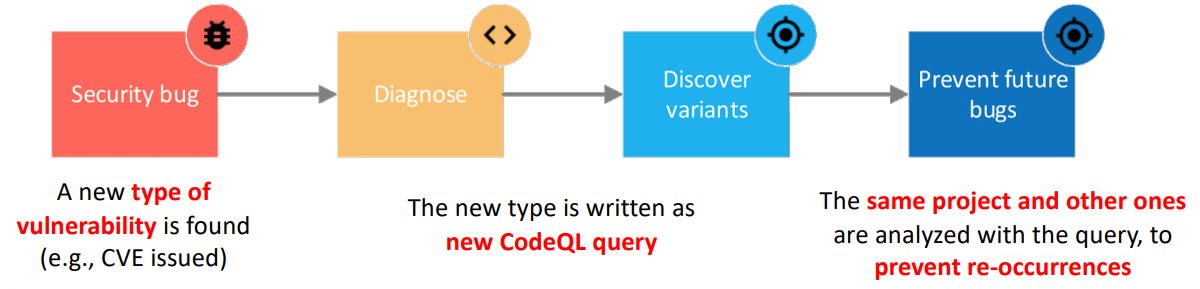
\includegraphics[width=1\linewidth]{img/capitolo7/codeql.png}
    \label{fig:codeql}
\end{figure}

Il linguaggio CodeQL è dichiarativo e orientato agli oggetti, strutturato in tre 
clausole primarie: \textbf{from} (dichiarazioni di variabili), \textbf{where} 
(condizioni logiche), e \textbf{select} (output desiderato).

Quando si analizza il codice con CodeQL, le query si dividono principalmente in due categorie:

\begin{itemize}
    \item \textbf{Alert Queries}: Servono a identificare punti specifici nel codice 
    che violano una regola o rappresentano una vulnerabilità. L'output di queste 
    query è solitamente un singolo nodo o una posizione nel codice (ad esempio, "qui 
    c'è un blocco vuoto" o "qui viene chiamata una funzione deprecata").
    \item \textbf{Path Queries}: Vengono utilizzate per le analisi più complesse, 
    come la \textit{Dataflow Analysis} e la \textit{Taint Analysis}. Invece di 
    restituire un singolo punto, tracciano un intero percorso del flusso di 
    informazioni da un punto di origine (\textit{source}) fino a un punto di 
    destinazione (\textit{sink}), permettendo di capire come i dati viaggiano 
    all'interno del programma.
\end{itemize}

\textbf{Alert Queries}

Il linguaggio CodeQL permette di scrivere query con livelli di astrazione crescenti, 
rendendo il codice estremamente riutilizzabile. Vediamo i tre approcci principali:

Esempio \textit{Base}:

\begin{lstlisting}
import java
from BlockStmt block
where block.getNumStmt() = 0
select block, "This block-statement is redundant."  
\end{lstlisting}

In questo esempio CodeQL scansiona il database chiedendo di trovare tutte 
le entità di tipo \textit{BlockStmt} (blocchi di codice tra parentesi graffe \{...\}) 
che contengono zero istruzioni interne.

Esempio con \textit{Predicato}: 

\begin{lstlisting}
import java
predicate isEmpty(BlockStmt block) {
    block.getNumStmt() = 0
}
from BlockStmt block
where isEmpty(block)
select block, "This block-statement is redundant."
\end{lstlisting}

In questo esempio, invece di scrivere la condizione direttamente nel \textit{where}, 
viene incapsulata nel predicato \textit{isEmpty}. La query cerca tutti i blocchi di 
istruzioni (\textit{BlockStmt}) e usa il predicato per filtrare solo quelli che 
contengono zero istruzioni.

Esempio con \textit{Classe}: CodeQL è orientato agli oggetti, si può definire una 
Classe per creare un sottoinsieme logico di un tipo esistente, usando un predicato 
al suo interno.

\begin{lstlisting}
import java
class EmptyBlock extends BlockStmt {
    EmptyBlock() { this.getNumStmt() = 0 }
}
from BlockStmt block
where block instanceof EmptyBlock
select block, "This block-statement is redundant."
\end{lstlisting}

Qui si crea una classe \textit{EmptyBlock} che estende \textit{BlockStmt}. La 
condizione che definisce l'appartenenza a questa classe è racchiusa nel 
costruttore (\textit{this.getNumStmt() = 0}). La query finale diventa: seleziona i 
blocchi che sono istanza di \textit{EmptyBlock}.

\textbf{Path Queries}

Sia la \textbf{Dataflow Analysis} che il \textbf{Taint Tracking} rientrano nella 
categoria delle Path Queries; il loro scopo è capire se un dato non attendibile che 
entra in un punto A (chiamato \textit{Source}) riesce a fluire fino a un punto B 
sensibile o pericoloso (chiamato \textit{Sink}) senza essere prima bloccato o pulito.

\textbf{1. Dataflow Analysis}

La \textbf{Dataflow Analysis} in CodeQL cerca le connessioni tra \textit{source} e \textit{sink} 
tracciando esclusivamente i flussi che preservano il valore esatto del dato 
(\textit{value-preserving flows}). Questo significa che è configurata per essere 
molto conservativa, con l'obiettivo principale di \textbf{evitare i falsi positivi}.

\begin{lstlisting}
String s = a.mySource(); // Source (Dato non sicuro)
String r = s + " test";  // Il dato viene modificato
b.mySink(r);             // Sink (Punto critico)
\end{lstlisting}

Se utilizziamo la Dataflow Analysis pura, CodeQL ignorerà questo percorso. Perché? 
Perché il valore originale di $s$ non è arrivato intatto al \textit{sink}; è stato 
concatenato con la stringa \textit{" test"}. Poiché il valore non è stato 
strettamente preservato, l'analisi si ferma per non rischiare di lanciare un falso 
allarme. Se invece il codice fosse stato semplicemente \textit{String r = s;}, la 
Dataflow Analysis avrebbe rilevato il flusso.

Vediamo dunque come si scrive la query:

\begin{lstlisting}
import java
import semmle.code.java.dataflow.DataFlow::DataFlow
from MethodCall a, MethodCall b, VarAccess arg
where a.getMethod().getName() = "mySource" and
      b.getMethod().getName() = "mySink" and
      arg = b.getAnArgument() and
      localFlow( exprNode(a),
                 exprNode(arg)
      )
select arg, "Data-flow found to mySink()"
\end{lstlisting}

Qui notiamo un dettaglio tecnico fondamentale: \textit{exprNode()}. CodeQL mantiene 
due mondi separati: l'AST (\textit{Abstract Syntax Tree}, che rappresenta la 
sintassi del codice) e il \textit{Data-Flow Graph} (il grafo logico di come 
fluiscono i dati). La funzione \textit{exprNode()} serve proprio a prendere un 
elemento sintattico dell'AST e convertirlo nel suo nodo corrispondente all'interno 
del grafo del flusso di dati, permettendo a \textit{localFlow} di verificare se sono connessi.

Specifichiamo che i predicati \textit{localFlow} e \textit{localTaint} compiono una 
\textbf{Local ("intra-procedural")} data flow; in questa tipologia i modelli circolano 
all'interno di una singola funzione e per questo sono leggeri. I predicati \textit{isSource} e 
\textit{isSink} compiono una \textbf{Global ("inter-procedural")} data flow; in tale
tipologia i modelli circolano tra le varie chiamate di funzione e per questo il calcolo 
può risultare più oneroso.

\begin{figure}[H]
    \centering
    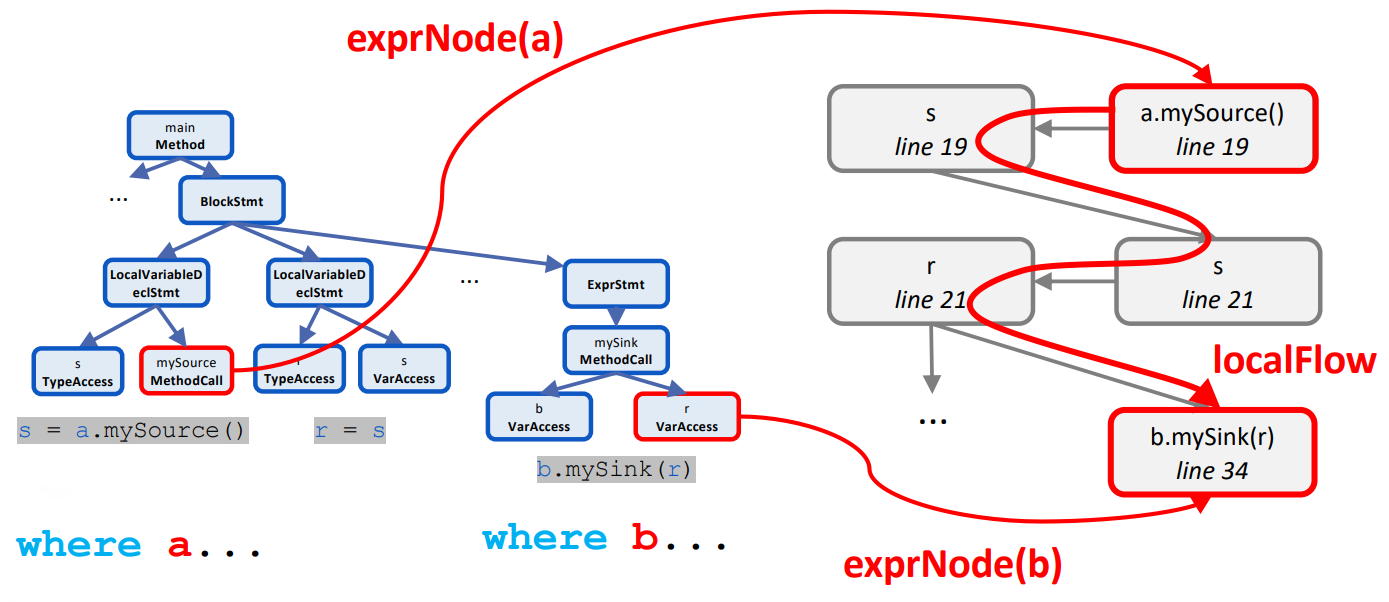
\includegraphics[width=1\linewidth]{img/capitolo7/astTodfg.png}
    \label{fig:astTodfg}
    \caption{Da AST a DFG}
\end{figure}

\textbf{2. Taint Tracking}

Il \textbf{Taint Tracking} fa un passo oltre: segue la "contaminazione" del dato, 
tracciando anche i flussi che non preservano il valore (\textit{non-value-preserving flows}). 
Se una variabile tocca un dato contaminato (\textit{tainted}), viene considerata 
contaminata a sua volta. È un approccio meno conservativo che accetta di generare 
qualche falso positivo in più, pur di scovare vulnerabilità reali sfuggenti.

Con lo stesso codice di prima:

\begin{lstlisting}
String s = a.mySource(); // Source (Dato non sicuro)
String r = s + " test";  // Il dato viene modificato
b.mySink(r);             // Sink (Punto critico)
\end{lstlisting}

Se usiamo il Taint Tracking, CodeQL rileverà il percorso. Anche se $s$ è stato 
modificato, la variabile $r$ è stata chiaramente "influenzata" da $s$ e quindi 
risulta contaminata. Quando $r$ arriva a \textit{mySink()}, scatta l'allarme.

La struttura della query è quasi identica a quella precedente, ma utilizza un modulo diverso:

\begin{lstlisting}
import java
import semmle.code.java.dataflow.DataFlow::DataFlow
import semmle.code.java.dataflow.TaintTracking
from MethodCall a, MethodCall b, VarAccess arg
where a.getMethod().getName() = "mySource" and
      b.getMethod().getName() = "mySink" and
      arg = b.getAnArgument() and
      TaintTracking::localTaint(
                                exprNode(a),
                                exprNode(arg)
                                )
select b, "Taint propagation found to mySink()"
\end{lstlisting}

\textbf{3. Taint Tracking Globale e Configurazioni Custom}

I metodi \textit{localFlow} e \textit{localTaint} sono utili ma limitati, poiché 
guardano solo all'interno di una singola funzione. Le vulnerabilità vere, però, 
viaggiano attraverso molte chiamate a funzioni diverse (analisi "inter-procedurale" 
o Globale).

Per fare un \textbf{Taint Tracking Globale}, CodeQL richiede di scrivere una 
configurazione personalizzata, creando un modulo che implementa \textit{DataFlow::ConfigSig}. 
In questa configurazione si deve definire esplicitamente le regole del gioco:

\begin{lstlisting}
public static void main(String[] args) {
    MyClassA a = new MyClassA();
    MyClassB b = new MyClassB();
    String s = a.mySource();
    String r = s + " test";
    boolean match = Pattern.matches("^[a-zA-Z]$", r);
    if(match == false) {
        System.out.println("Taint detected!");
        System.exit(1);
    }
    b.mySink(r);
}
\end{lstlisting}

\begin{enumerate}
    \item \textbf{isSource}: Definisce da dove parte la contaminazione. Nell'esempio, 
    la query cerca le chiamate al metodo \textit{mySource()} della classe \textit{MyClassA}.
    \item \textbf{isSink}: Definisce dove non vogliamo che i dati contaminati arrivino.
    Nell'esempio, il sink è definito come l'argomento passato al metodo \textit{mySink()} 
    della classe \textit{MyClassB}.
    \item \textbf{isBarrier}: Definisce un nodo che "ripulisce" il dato, bloccando 
    il taint tracking. Nell'esempio, il codice usa un'espressione regolare (\textit{Pattern.matches(...)}) 
    per validare l'input. Il predicato \textit{isBarrier} istruisce CodeQL a smettere 
    di tracciare la variabile se passa attraverso questo controllo, evitando così un 
    falso positivo.
\end{enumerate}

Mentre prima usavamo \textit{exprNode()} per passare dall'AST al Grafo dei Dati, 
all'interno di questa configurazione globale vediamo l'uso inverso di \textit{asExpr()}. 
I predicati \textit{isSource}, \textit{isSink} e \textit{isBarrier} ricevono in input 
dei nodi del Grafo dei Dati (\textit{DataFlow::Node}), ma per capire se quel nodo 
rappresenta la chiamata a \textit{mySource()} o \textit{mySink()}, dobbiamo prima 
convertirlo indietro in un nodo sintattico dell'AST usando \textit{node.asExpr()}. 
Solo allora possiamo ispezionarne il nome, la classe di appartenenza o gli argomenti.

\begin{lstlisting}
module MyConfig implements DataFlow::ConfigSig {
    predicate isSource(DataFlow::Node n) { ... }
    predicate isSink(DataFlow::Node n) { ... }
    predicate isBarrier(DataFlow::Node n) { ... }
    ...
}
\end{lstlisting}